% --------------------------------------------------------------
% This is all preamble stuff that you don't have to worry about.
% Head down to where it says "Start here"
% --------------------------------------------------------------
 
\documentclass[12pt]{article}
 
\usepackage[margin=1in]{geometry} 
\usepackage{amsmath,amsthm,amssymb}
\usepackage{graphicx}
\usepackage{epstopdf}

\newcommand{\N}{\mathbb{N}}
\newcommand{\Z}{\mathbb{Z}}
 
\newenvironment{theorem}[2][Theorem]{\begin{trivlist}
\item[\hskip \labelsep {\bfseries #1}\hskip \labelsep {\bfseries #2.}]}{\end{trivlist}}
\newenvironment{lemma}[2][Lemma]{\begin{trivlist}
\item[\hskip \labelsep {\bfseries #1}\hskip \labelsep {\bfseries #2.}]}{\end{trivlist}}
\newenvironment{exercise}[2][Exercise]{\begin{trivlist}
\item[\hskip \labelsep {\bfseries #1}\hskip \labelsep {\bfseries #2.}]}{\end{trivlist}}
\newenvironment{reflection}[2][Reflection]{\begin{trivlist}
\item[\hskip \labelsep {\bfseries #1}\hskip \labelsep {\bfseries #2.}]}{\end{trivlist}}
\newenvironment{proposition}[2][Proposition]{\begin{trivlist}
\item[\hskip \labelsep {\bfseries #1}\hskip \labelsep {\bfseries #2.}]}{\end{trivlist}}
\newenvironment{corollary}[2][Corollary]{\begin{trivlist}
\item[\hskip \labelsep {\bfseries #1}\hskip \labelsep {\bfseries #2.}]}{\end{trivlist}}
 
\begin{document}
 
% --------------------------------------------------------------
%                         Start here
% --------------------------------------------------------------
 
%\renewcommand{\qedsymbol}{\filledbox}
 
\title{What does CG give us in nonconvex problems?}%replace X with the appropriate number
% \author{Chenxin} %if necessary, replace with your course title
\date{\vspace{-10ex}}
\maketitle
 

\section{The problem and the data}


I only focus on two simple networks and two sets of one dimensional data.


Network 1 (N1) has the $1-2-1$ structure, thus has 7 parameters in total. Network 2 (N2) has the $1-1-1$ structure, thus has $4$ parameters in total. I tried linear, Relu, sigmoid as three activation functions and square loss as the loss function. However, for simplicity, here all the results are based on sigmoid activation function only. Figure~\ref{fig:n} shows the network structure.
\begin{figure}[h]
\centering
\includegraphics[width=6cm]{n1}
\includegraphics[width=6cm]{n2}
\caption{N1 (left) and N2 (right).}
\label{fig:n}
\end{figure}

Dataset one (D1) contains $4$ samples, two in each class. Dataset two (D2) contains $20$ samples, $10$ in each class. Figure~\ref{fig:d}  shows the distribution of both of them.
\begin{figure}[h]
\includegraphics[width=8cm]{data1.eps}
\includegraphics[width=8cm]{data2.eps}
\caption{D1 (left) and D2 (right). Red samples have $1$-label, while green samples have $0$-label.}
\label{fig:d}
\end{figure}

Notice that for D1, N1 should be able to achieve $100\%$ accuracy after training, but D2 is a rather ``difficult'' dataset for both these two networks.

\section{Can CG give a better direction than gradient?}

Here we focus on N1 only. We choose $200$ random points in ${\bf R}^7$ for initializing parameters. For each point, the gradient $d_{gd}$ and the results of CG steps $d_{cg}$ are computed. After line search, we are able to obtain two updated points and their objective values, i.e., $f_{gd}$ and $f_{cg}$. We record the ratio
$$ r:=\frac{f_{gd} - f_0}{f_{cg} - f_0 } $$
to measure the ``quality'' of two updates, where $f_0$ is the original objective value before taking any updates. Thus, $r>1$ means negative gradient could lead to more decreasing on objective value than a CG step, and vice versa.

The only difference between CG implemented here and traditional CG is, here if $\alpha<0$, we will terminate CG loops and return the negative curvature direction as output. 

The number of maximal CG iterations is tuned from $1$ to $5$.

We apply backtrack line search in both gradient steps and CG steps. The initial step size is $10$ and multiplier on it is $0.5$ if the iteration has to go on. However, for CG steps, we need to flip the sign of step size in each line search iterations since the direction may not be a descent direction. 
 
\begin{figure}[h]
\includegraphics[width=8cm]{CGD1.eps}
\includegraphics[width=8cm]{CGD2.eps}
\caption{Results for D1 (left) and D2 (right).}
\label{fig:CGvsGD}
\end{figure}

The figures above are two bar plots showing, by setting different maximal iterations for CG, the percentages of $r>1$ and $r<1$. The observation is that, running more than $3$ iterations of CG does not change the results at all. The reason is that CG will find a negative curvature direction in first $3$ iterations in all cases. 

Another observation is, by allowing CG to take more iterations, the outputs of CG have lower chance to beat gradient direction. Therefore, I guess the reason here is those negative curvature directions cannot provide much decrease on objective.


\section{How is leftmost eigenvector of Hessian?}

Here we consider to use leftmost eigenvector as the direction to make updates. In particular, at any point, if the leftmost eigenvalue of Hessian is less than $0$, then we use left most eigenvector to do line search. If it is greater than $0$, then we use the output of CG with $5$ as maximal number of iterations. (It is worthwhile to note that for N1 and both datasets, as far as I see, all the random points have negative leftmost eigenvalue in the Hessian.)

By running the experiments again, I found there are $\mathbf{26\%}$ cases which lead to $r>1$ for D1 and $\mathbf{19\%}$ cases leading to $r>1$ for D2. The results indicate that leftmost eigenvector of Hessian could be a direction that has larger chance to lead to a larger decrease in objective than gradient. This also suggest that the negative curvature directions returned by CG is not ``negative enough'' since the product $p^TA p$ (even though it is negative) can be rather close to $0$.

\begin{figure}[h]
\includegraphics[width=8cm]{ncd1.eps}
\includegraphics[width=8cm]{ncd2.eps}
\caption{Results for D1 (left) and D2 (right).}
\label{fig:CGvsGD}
\end{figure}

\section{Visualization of these directions on N2}

From now on, we consider to build some visualization on N2. Note that we will fix the value of two biases so that there will be only 2 weights as parameters.

\begin{figure}[h]
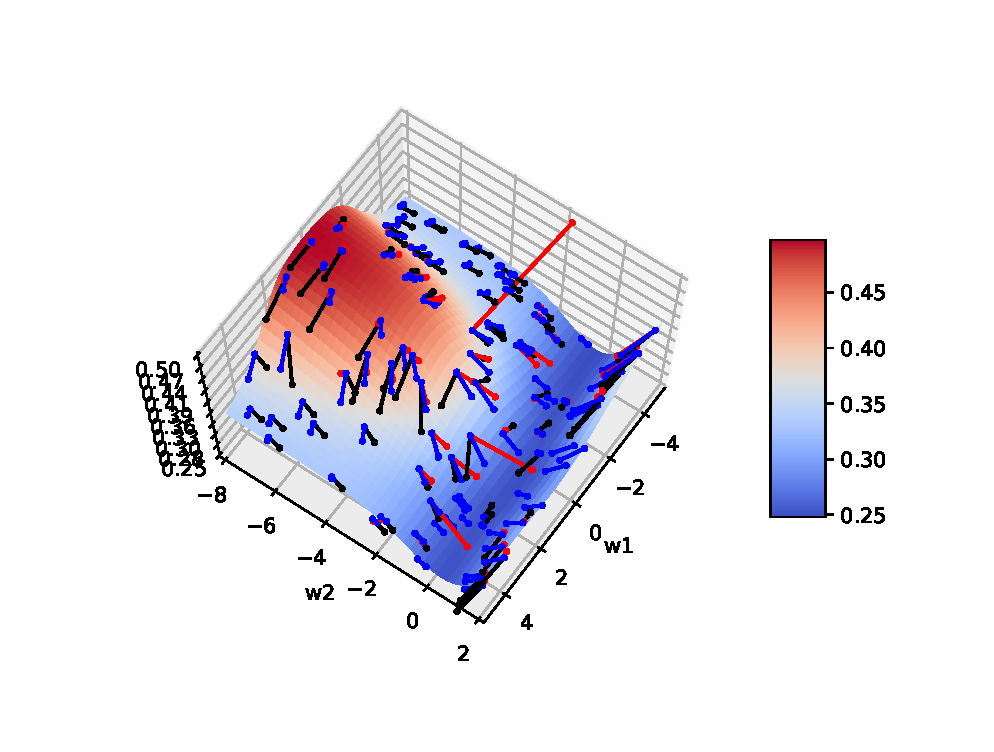
\includegraphics[width=15cm]{2w.eps}
\label{fig:CGvsGD}
\end{figure}

\section{Using three directions as three algorithms for training.}

Figure~\ref{fig:3m} is a screenshot of running each algorithms for $100$ iterations, starting with $10$ different initial points. 
\begin{figure}[h]
\includegraphics[width=16cm]{threeM}
\caption{}
\label{fig:3m}
\end{figure}
\end{document}